\documentclass[12pt, letterpaper]{article}
\usepackage[margin=1in]{geometry}
\usepackage{amsmath,amsthm,array, amssymb,amsfonts, enumitem, fancyhdr, color, comment, graphicx, environ}

\author{Val Anthony Balagon}
\date{January 2019}
\title{Chapter 4: Orthogonality}

%User commands
\newcommand{\R}[1]{$\mathbb{R}^{#1}$}
\newcommand{\Vector}[1]{$\textbf{#1}$}
\newcommand{\V}[1]{\textbf{\textit{#1}}}

\newcommand{\A}{$A$}
\newcommand{\x}{\textbf{\textit{x}}}
\newcommand{\B}{\textbf{\textit{b}}}
\newcommand{\system}{\textbf{\textit{\A \x = \B}}}
\newcommand{\nullsystem}{\textbf{\textit{\A\x}} = \textbf{0}}
\newcommand{\DefinitionSpace}{\vspace{15px}}


\newtheorem*{remark}{Remark}
\theoremstyle{definition}
\newtheorem{definition}{Definition}[section]
\newtheorem{example}{Example}
\newtheorem{theorem}{Theorem}

\newcommand*{\vertbar}{\rule[-1ex]{0.5pt}{2.5ex}}



\newenvironment{problem}[2][Problem]{\begin{trivlist}
		\item[\hskip \labelsep {\bfseries #1}\hskip \labelsep {\bfseries #2.}]}{\end{trivlist}}



\begin{document}
	\maketitle
	\begin{abstract}
		This chapter focuses on the orthogonality of the four subspaces, projections, and least squares approximations.
	\end{abstract}

\section{Orthogonality of the Four Subspaces}

	Two vectors are orthogonal when their dot product is zero $\V{v} \cdot \V{w} = \V{v}^T \V{w} = 0$. This chapter will revolve around orthogonal subspaces, orthogonal bases, and orthogonal matrices.
	
	\DefinitionSpace
	\begin{definition}
		Orthogonal vectors have the following properties:
		\renewcommand{\theenumi}{\roman{enumi}}
		
		\begin{enumerate}[leftmargin=2\parindent]
			\item $\V{v}^T \V{w} = 0$
			\item $||\V{v}||^2 + ||\V{w}||^2 = ||\V{v} + \V{w}||^2 \rightarrow \V{v}^T\V{v} + \V{w}^T\V{w} = (\V{v}+\V{w})^T(\V{v}+\V{w})$
		\end{enumerate}	
	
	\end{definition} 	
	
	\DefinitionSpace
	\begin{remark}
		The zero vector is orthogonal to any vector.
	\end{remark}
	

	\DefinitionSpace
	\begin{remark}
		The subspaces have orthogonal properties. 
		\begin{enumerate}
			\item \textbf{The rowspace $C(A^T)$ is perpendicular to the nullspace $N(A)$}. Every row of $A$ is perpendicular to the solution of $A\V{x} = \textbf{0}$.
			\item \textbf{The column space $C(A)$ is perpendicular to the left nullspaces $N(A^T)$}. When $\V{b}$ is outside of the column space when we're trying to solve for $A\V{x} = \V{b}$, then this nullspace of $A^T$ comes into its own. It contains the error $\V{e} = \V{b} - A\V{x}$ in the least-squares solution.
		\end{enumerate}
	\end{remark}
	\DefinitionSpace
	

	\begin{definition}
		Two subspaces \V{V} and \V{W} of a vector space are orthogonal if every vector \V{v} in \V{V} is perpendicular to every vector \V{w} in \V{W}.
		\renewcommand{\theenumi}{\roman{enumi}}
		
		\begin{equation*}
			\V{v}^T \V{w} = 0 \text{ for all \V{v} in \V{V} and all \V{w} in \V{W}.}
		\end{equation*}
	\end{definition} 	
	\DefinitionSpace
	
	
	\begin{theorem}
	Every vector \V{x} in the nullspace is perpendicular to every row of $A$, because $A\V{x} = \textbf{0}$. The nullspace $N(A)$ and the row space $C(A^T)$ are orthogonal subspaces of \R{n}.
	
		\begin{equation*}
			A \V{x} = \begin{bmatrix} \text{row 1} \\ \vdots \\ \text{row m} \end{bmatrix} \begin{bmatrix} x_1 \\ \vdots \\ x_n \end{bmatrix} = \begin{bmatrix} 0 \\ \vdots \\ 0 \end{bmatrix}
		\end{equation*}
		\begin{gather*}
			C_1(\text{row}_1^T) = 0 \\
			C_2(\text{row}_2^T) = 0 \\
			\vdots \\
			C_m(\text{row}_m^T) = 0
		\end{gather*}
	\end{theorem}
	\noindent (row 1) $\cdot \V{x}$ is zero and (row $m) \cdot \V{x}$ is also zero. Every row has a zero dot product with \V{x}. Then \V{x} is perpendicular to every combination of the rows. \textbf{The whole row space $C(A^T)$ is orthogonal to $N(A)$. }
	\DefinitionSpace
	
	
	\begin{proof}
		The vectors in the row space are combinations of $A^T \V{y}$ of the rows. We take the dot product of $A^T \V{y}$ with any \V{x} in the nullspace.
			\begin{gather*}
				\V{x} \cdot (A^T \V{y}) = \V{x}^T (A^T \V{y}) = (A\V{x})^T \V{y} = 0^T \V{y} = 0
			\end{gather*}
	\end{proof}
	\DefinitionSpace
	
	\begin{example}
		The rows of $A$ are perpendicular to $\V{x} = (1,1,-1)$ in the nullspace:
		\begin{gather*}
			A\V{x} = \begin{bmatrix} 1&3&4 \\ 5&2&7\end{bmatrix} \begin{bmatrix} 1 \\ 1 \\ -1 \end{bmatrix} = \begin{bmatrix} 1+3-4 \\ 5+2-7 \end{bmatrix} = \begin{bmatrix} 0\\ 0 \end{bmatrix}
		\end{gather*}
		In this example, the column space is all of \R{2}. The nullspace of $A^T$ is the zero vector. The column space of $A$ and the nullspace of $A^T$ are always orthogonal subspaces.
	\end{example}


	\begin{theorem}
		Every vector \V{y} in the nullspace of $A^T$ is perpendicular to every column of $A$. The left nullspace $N(A^T)$ and the column space $C(A)$ are orthogonal in \R{m}.
	\end{theorem}

	\begin{proof}
		The nullspace of $A^T$ is orthogonal to the row space of $A^T$, which is the column space of $A$.
		
		\begin{gather*}
			A^T\V{y} = \begin{bmatrix} \text{(column 1)}^T \\ \vdots \\ \text{(column n)}^T \end{bmatrix} \begin{bmatrix} y_1 \\ \vdots \\ y_m \end{bmatrix} = \begin{bmatrix} 0 \\ \vdots \\ 0 \end{bmatrix}
		\end{gather*}
	\end{proof}
	
	\DefinitionSpace
	\begin{theorem}
		If a vector \V{v} is orthogonal to itself, then \V{v} is the zero vector.
	\end{theorem}
	\DefinitionSpace
	
	\begin{figure}[h!]
		\centering
		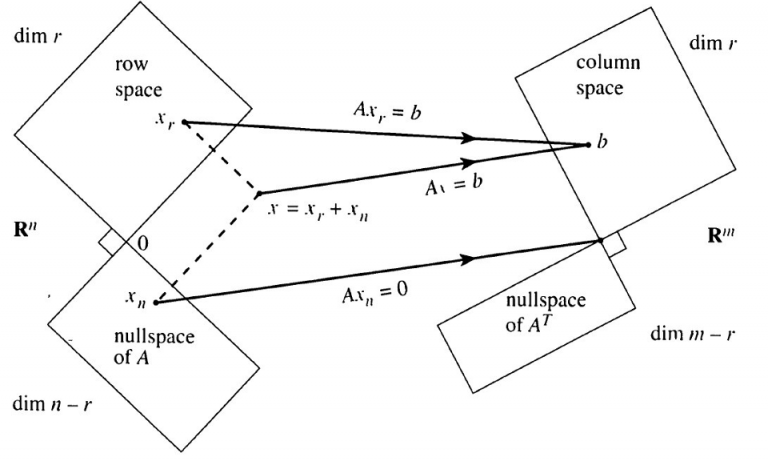
\includegraphics[scale=0.5]{4-subspaces.png}
		\caption{The Four Subspaces. There are two pairs of orthogonal subspaces.}
		\label{4subs}
	\end{figure}

	\begin{theorem}
		Fundamental Theorem of Linear Algebra, Part 2: \\
		\quad\textbf{$N(A)$ is the orthogonal complement of the row space $C(A^T)$ in \R{n}. \\
		\quad $N(A^T)$ is the orthogonal complement of the column space $C(A)$ in \R{m}.}
	\end{theorem}\DefinitionSpace 

	Things to note from Figure \ref{4subs}
	\begin{enumerate}
		\item When $A$ multiplies to $\V{x} = \V{x}_r + \V{x}_n$, it goes to \V{b} which is in the column space.
		\item When $A$ multiplies to $\V{x}_r$, it goes to \V{b} which is also in the column space.
		\item When $A$ multiplies to $\V{x}_n$, the nullspace component goes to \textbf{0}.
	\end{enumerate}
	
	
	
\subsection{Combining Bases from Subspaces}
	\begin{theorem}
		Any independent vectors in \R{n} must span \R{n}. So they are a basis.\\
		Any $n$ vectors that span \R{n} must be independent. So they are a basis
	\end{theorem}\DefinitionSpace 
	
	\begin{theorem}
		If the $n$ columns of $A$ are independent, they span \R{n}. So $A\V{x} = \V{b}$ is solvable.\\
		If the $n$ columns span \R{n}, they are independent. So $A\V{x} = \V{b}$ has only one solution.
	\end{theorem}\DefinitionSpace 
	
	
	
	
\section{Problems}


	\begin{problem}{1.1}
		asd
	\end{problem}
	
	\begin{proof}[Solution]
		soln
	\end{proof}
	
	
	
	
	
	
	


\end{document}